% !TEX root = ../main.tex

\section{Conclusions}

The reduced-order models discussed in this report do not give as much detail as full three-dimensional simulations; however, they provide reasonable results in a timely manner without requiring expensive computational resources. Such models lend themselves well to process modeling, design of experiments, and rapic prototyping tasks.

\section{Hardware requirements}

The reduced order models in this report are developed and executed on a MacBook Pro laptop. See the list below for hardware specifications.

\begin{itemize}
    \item MacBook Pro, 16-inch, 2019 model
    \item 2.3 GHz 8-core Intel i9 CPU
    \item 32 GB 2667 MHz DDR4 memory
    \item 4 GB AMD Radeon Pro 5500M GPU
    \item macOS Big Sur version 11.6
\end{itemize}

\section{Source code and web application}

Source code for this project is available on GitHub at the link provided below. See the README markdown document in the repository for more information.

\begin{itemize}
    \item \url{https://github.com/wigging/fcic-pyrolysis}
\end{itemize}

A web application was developed based on the biomass compositional work discussed in this report. The application is an online tool for calculating biomass composition from ultimate and chemical analysis data. The resulting composition can be used with reactor models that utilize the Debiagi et al. kinetics scheme \cite{Debiagi-2018}. The application and its source code are available at the URLs given below. A screenshot of the application in a browser window is shown in Figure \ref{fig:webtool}.

\begin{itemize}
    \item \url{https://share.streamlit.io/wigging/biocomp/main/app.py}
    \item \url{https://github.com/wigging/biocomp}
\end{itemize}

\begin{figure}[H]
    \centering
    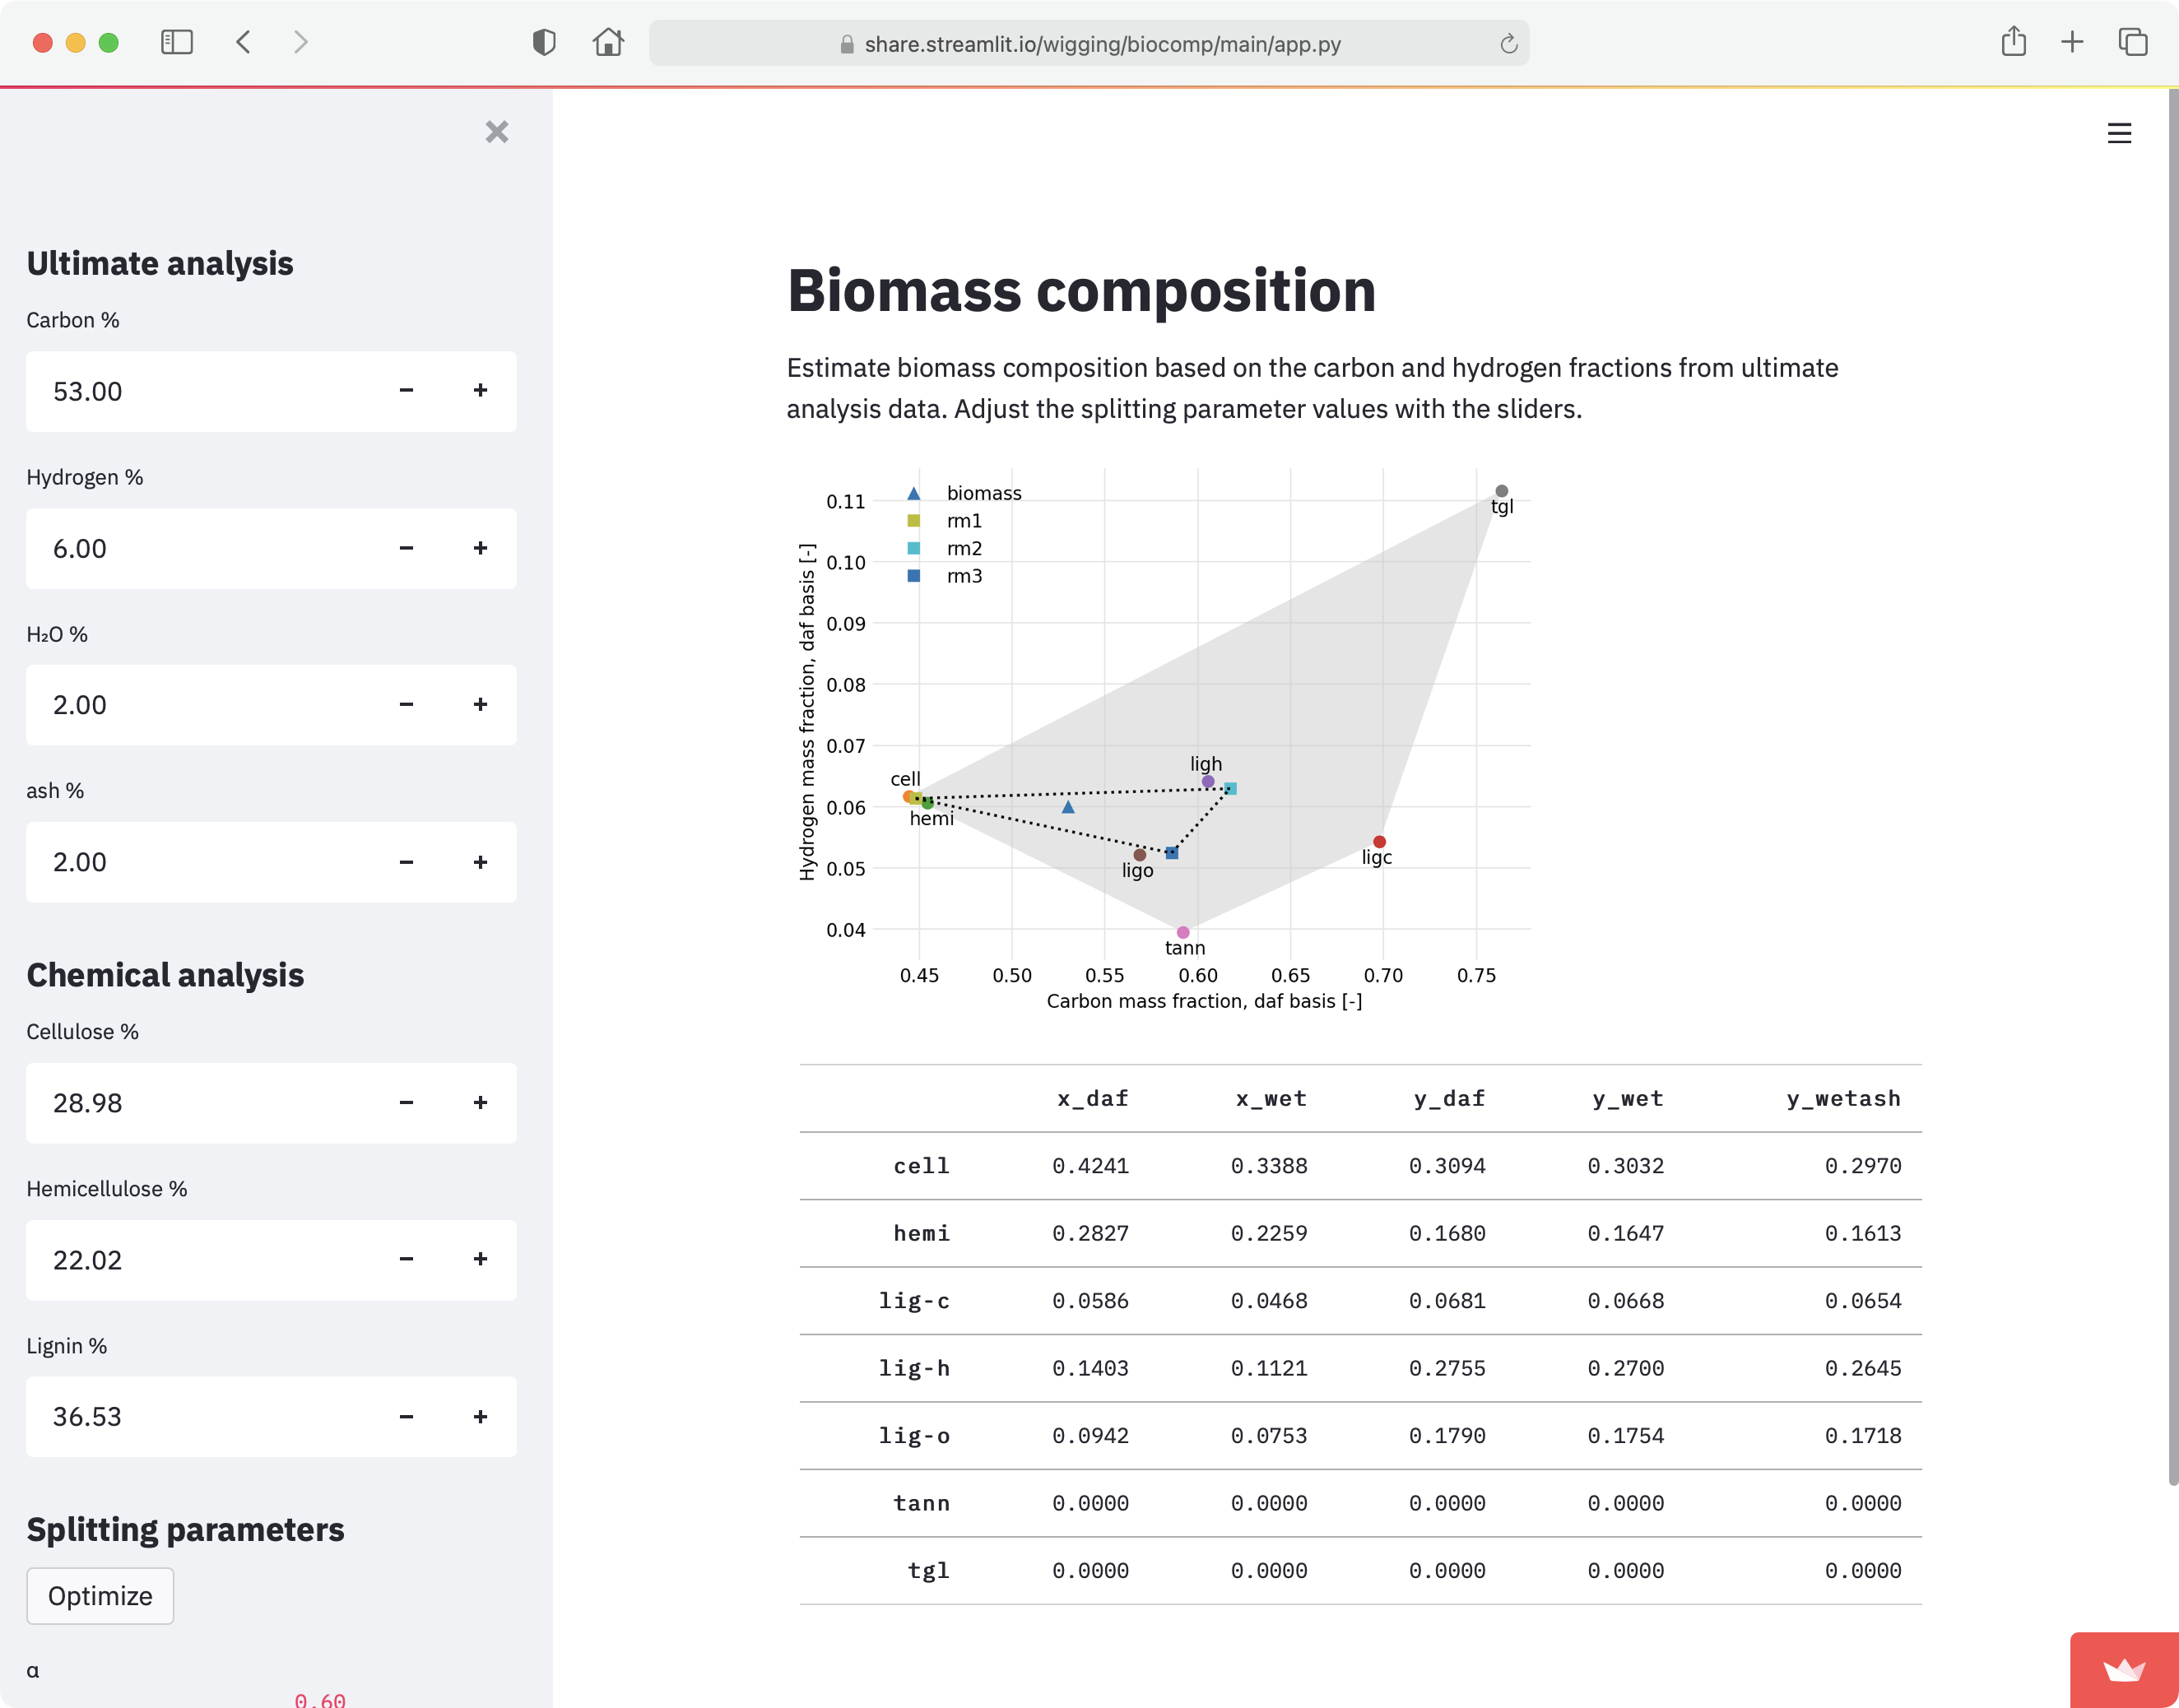
\includegraphics[width=0.8\textwidth]{figures/webtool.png}
    \caption{An online tool to estimate biomass composition from ultimate and chemical analysis data.}
    \label{fig:webtool}
\end{figure}
